\section{Requirements} \label{sec:Requirements}

\subsection{Business Case} \label{sec:Requirements.BusinessCase}
Any personal accounting system should be able to provide accurate and relevant
summaries of an individual's financial status. In order to do this, the user
needs to be able to supply the system with the necessary data, so that it can
be analysed and properly converted into knowledge.

The scope of the personal finance system developed for this project must
include a feature to allow a user to upload their bank and credit card
statements into it. Each transaction should be classified based on categories
which the user will create. The user should then be able to visualise a summary
of their income and expenditure by category and period, which should allow them
to have a concise and clear visibility of how much they have earned and spent
over any period of time. The category must be handled with care -- there should
not be a case where a user deletes a category and then all the entries in a
period are lost with it, but if a user wants to change the name of a category
they should be free to do so.

Since there may be other sources of income which the user may want to
categorise (such as breakdowns of cash transactions from pocket money), a
feature to allow for manual entries should also be made available. The user can
declare a lump sum, and then break it down among categories. The option should
allow them to choose whether the transaction is a credit or a debit from a
specific category, and then provide the corresponding debit or credit to a
category of their choice. For example, if the user withdraws \pounds50, and
spends half of it on weekly shopping and the other half on a cinema ticket,
they should be able to `credit' (withdraw) \pounds50 from the \emph{Bank}
category, and then `debit' \pounds25 to both \emph{Weekly Shopping} and
\emph{Entertainment} categories.

Once the system has enough data, it should be able to calculate a simple budget
and display it for the user. The budget can be a simple average of income and
expenditure over a long enough period of time, projected over the future
month/year -- it would only be used as a guideline for the user, anyway.

\subsection{Functional Requirements} \label{sec:Requirements.FunctionalRequirements}

Based on the description above, a few functional requirements were identified.
They are represented in the diagram on section
\ref{sec:Requirements.FunctionalRequirements.UseCaseDiagram} and the list,
wireframes and activity diagrams on section
\ref{sec:Requirements.FunctionalRequirements.UseCaseList}.

\subsubsection{Use Case Diagram} \label{sec:Requirements.FunctionalRequirements.UseCaseDiagram}
Use case diagrams are UML constructs which were developed by Jacobson et al.
(1992, cited \cite[][p.~154]{bennett2010object}). The use case diagram on
Figure \ref{fig:UseCaseDiagram} is used to illustrate the functional
requirements identified for this project:
\begin{figure}[ht!]
  \begin{center}
    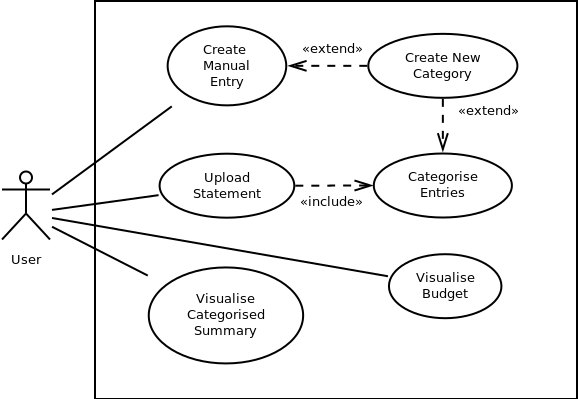
\includegraphics[width=14cm]{./contents/img/Use_Case_Diagram.png}
  \end{center}
  \caption{Use Case Diagram}
  \label{fig:UseCaseDiagram}
\end{figure}
\FloatBarrier



\subsubsection{Use Case List} \label{sec:Requirements.FunctionalRequirements.UseCaseList}
Table \ref{tab:UseCaseDescriptions} lists the descriptions for the use cases
listed above:
\begin{table}[ht!]
  \centering
  \begin{tabular}{|p{4cm}|p{12cm}|}
    \hline
    \textbf{Use Case}&\textbf{Description}\\
    \hline
    Upload Statement&The user must be able to upload a list of their
                     financial transactions, most likely their bank
                     or credit card statements, in a valid format, and all
                     entries should be categorised based on specific patterns\\
                    &\emph{Includes}: Categorise Entries\\
    \hline
    Create Manual Entry&The user should be able to create a manual transaction for
                        income or expenditure, include a date, amount and
                        description, and classify it among existing categories
                        or create new ones in the
                        process\\
                        &\emph{Extends}: Create Category\\
    \hline
    Visualise Categorised Summary&The user must be able to visualise
                                  a summary of their income and expenditure
                                  over a period of time\\
    \hline
    Calculate Budget&The user must be able to visualise a budget for future
                     periods based on their income and expenditure data 
                     already entered\\
    \hline
    Categorise Items&Analyse the current entry and assign it to a category\\
                    &\emph{Extends}: Create Category\\
    \hline
    Create Category&Creates a new category with the name suggested by the
                        user\\

    \hline
  \end{tabular}
  \caption{Use Case Descriptions} \label{tab:UseCaseDescriptions}
\end{table}
\FloatBarrier


\subsubsection{Designing the User Experience with Wireframes}
The wireframe below (Figure \ref{fig:Wireframe.CreateManualEntry}) was created
to better illustrate the \emph{Manual Entry} requirement from the point of view
of the user. It shows an example of an entry for a laptop and a licence for a
proprietary operating system, which can then be broken down among different
categories. The user has the option to use the percentage or the amount boxes
in order to provide a breakdown, and they can also add new lines if more than
one is required -- the example shows two lines, but the default would be one.
Under the category search box, if the user types a category name that does not
exist they will be asked if they want to create a new one:
\begin{figure}[ht!]
  \begin{center}
    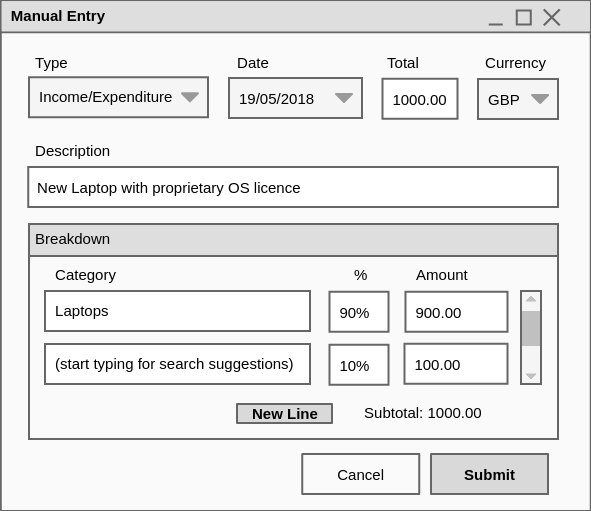
\includegraphics[width=14cm]{./contents/img/Wireframe_-_Manual_Entry.png}
  \end{center}
  \caption{User interface wireframe for \emph{Create Manual Entry} use case}
  \label{fig:Wireframe.CreateManualEntry}
\end{figure}
\FloatBarrier

And in order to better understand the relationship between \emph{Upload
Statement} and \emph{Categorise Entries}, the activity diagram below (Figure
\ref{fig:AD.CategoriseEntries}) was developed:
\begin{figure}[ht!]
  \begin{center}
    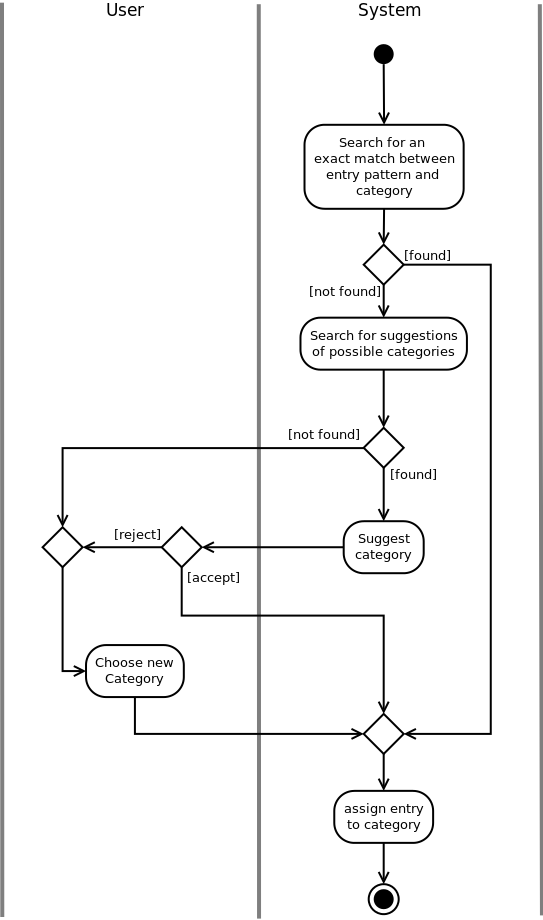
\includegraphics[width=11cm]{./contents/img/Activity_Diagram_-_Categorise_Entries.png}
  \end{center}
  \caption{}
  \label{fig:AD.CategoriseEntries}
\end{figure}
\FloatBarrier

At the first few iterations, in order to provide a minimum viable product, the
process of categorisation will be a blocking one consisting of multiple calls
being made to the process above -- for each call, the process will block awaiting
user input when a category is not found. However, there are plans for future
iterations where this process could be optimised by concurrency, and if there
is enough time a more appropriate interface will be built for such a case.

The initial interface for uploading a statement should be a simple one, such as
the one below
(\ref{fig:Wireframe.UploadStatement}), and at least initially the interface for
manual entry will be used whenever user input is required:
\begin{figure}[ht!]
  \begin{center}
    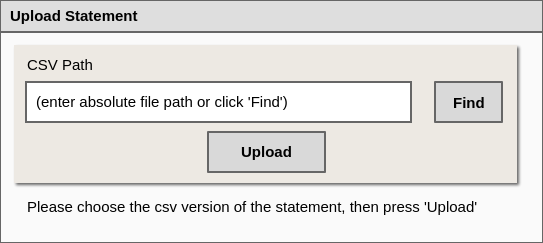
\includegraphics[width=12cm]{./contents/img/Wireframe_-_Upload_Statement.png}
  \end{center}
  \caption{}
  \label{fig:Wireframe.UploadStatement}
\end{figure}
\FloatBarrier

Below (Figure \ref{fig:Wireframe.VisualiseCategorisedSummary}) is also a
wireframe illustrating the GUI for \emph{Visualise Categorised Summary}. The
user should have an option to select the dates and, if they only want to see
one category, the category itself:
\begin{figure}[ht!]
  \begin{center}
    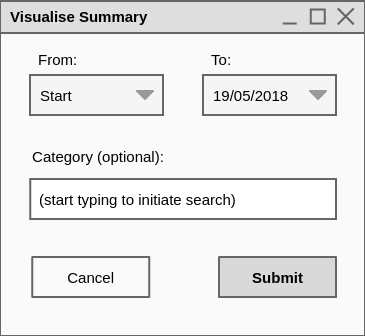
\includegraphics[width=8cm]{./contents/img/Wireframe_-_Visualise_Summary.png}
  \end{center}
  \caption{}
  \label{fig:Wireframe.VisualiseCategorisedSummary}
\end{figure}
\FloatBarrier

The dates field should allow them both to type a date or choose it from a drop
down calendar. If no values are entered, the system will return a summary of
all categories on the system.


\subsection{Non-Functional Requirements} \label{sec:Requirements.NonFunctionalRequirements}
At this iteration, no significant non-functional requirements were identified,
so they were not included in this report.
